\documentclass{aleph-revista}

\usepackage{tikz}           
\usepackage{aleph-comandos} 
\usepackage{multicol}    
\usepackage{indentfirst}
\usepackage{cleveref}
\usepackage{circuitikz}
\usepackage{graphicx}
\usepackage{listings}
\usepackage{xcolor}
\usepackage{tikz-dimline}
\usetikzlibrary{arrows,calc,patterns,decorations.markings,arrows.meta,quotes}

\definecolor{commentgreen}{RGB}{2,112,10}
\definecolor{eminence}{RGB}{108,48,130}
\definecolor{weborange}{rgb}{0.58,0,0.82}
\definecolor{frenchplum}{RGB}{129,20,83}

\lstset {
    language=Python,
    frame=tb,
    tabsize=4,
    showstringspaces=false,
    numbers=left,
    upquote=true,
    commentstyle=\color{commentgreen},
    keywordstyle=\color{eminence},
    stringstyle=\color{red},
    basicstyle=\small\ttfamily,
    emphstyle={\color{blue}},
    escapechar=\&,
    classoffset=1,
    otherkeywords={>,<,.,;,-,!,=,~},
    morekeywords={>,<,.,;,-,!,=,~},
    keywordstyle=\color{weborange},
    classoffset=0,
}
% \graphicspath{{figures/}}

\titulo{Exercício Escrito 02}
\tituloingles{Método das Imagens: Capacitâncias Parciais}

\autor{%
  Natanael Magalhães Cardoso\textsuperscript{1}
}

\institucion{
\textsuperscript{1}%
  n$^{o}$ USP: 8914122
}

\fecha{19 de julho de 2021}

% \abstract{
%   Este relatório mostra uma solução computacional de um problema do eletromagnetismo com um algorítmo de diferenciação numérica, o Método das Diferenças Finitas. Aqui são expostos dois problemas onde as equipotenciais, as linhas de campo elétrico e o valor da resistência são calculados.
% }

\begin{document}
\membrete

\vspace{1em}

\section{Dados do Sistema}

\begin{table}[!h]
  \centering
  \caption{Tabela com os dados do problema}
  \label{tab:dados}
  \begin{tabular}{ccc}
    \toprule
    Variável & Expressão                                       &
    Valor (SI)                                                                                  \\
    \midrule
    $m$      & -                                               & 1                              \\
    $n$      & -                                               & 2                              \\
    $p$      & -                                               & 2                              \\
    $a$      & $\displaystyle 2.5\left( \frac{m}{4}+1 \right)$ & $3.125\times10^{-3} \text{ m}$ \\
    $d$      & -                                               & 0.3 m                          \\
    $h$      & $\displaystyle \frac{n}{2} + 10$                & 11 m                           \\
    $l$      & -                                               & 1000 m                         \\
    $D$      & $\displaystyle \frac{p}{4}+1$                   & 1.5 m                          \\
    \bottomrule
  \end{tabular}
\end{table}

\section{Matriz de Capacitâncias}
\subsection{Hipóteses}
\begin{enumerate}
  \item Pelos valores da Tabela \ref{tab:dados}, a seguinte relação é estabelecida: $2a \ll \min(d, D, \mathcal{H}_k)$, onde $a$ é o raio de cada linha de transmissão, $\mathcal{H}_k$ é a altura da linha $k$ em relação ao solo, $D$ é a distância horizontal entre as linhas e $d$ é a distância vertical entre as linhas. Como o diâmetro da linha é $\approx 50$ vezes menor que a menor grandeza mensionada, as linhas de transmissão serão simplificados por linhas de carga imagens (retas) usando o método das imagens.
  \item Um fio descarregado tem influência desprezível sobre o potencial produzido pelo outro.
  \item As linhas de carga são uniformimente carregadas com cargas $Q_i$ e $-Q_i$.
\end{enumerate}

\newpage
\subsection{Equação do potencial e da elastância}
O potencial $\varphi$ devido a duas linhas de carga de comprimento $l$ uniformemente carregadas com cargas $Q_i$ e $-Q_i$ é aproximado pela expressão \eqref{eq:1}.

\begin{equation}\label{eq:1}
  \varphi = \frac{\rho_L}{2\pi\varepsilon}\ln\left(\frac{r_-}{r_+}\right) \quad \overset{\rho_L=Q/l}{\Rightarrow} \quad \varphi = \frac{Q}{2\pi\varepsilon_{ar} l}\ln\left(\frac{r_-}{r_+}\right)
\end{equation}


Como a equação \eqref{eq:1} apresenta uma relação de $\varphi$ e $Q$. As elastâncias $S_{ki}$ serão calculadas pela relação $V_k/Q_i$, quando o eletrodo $k$ tem potencial $V_k$ e o eletrodo $i$ tem carga $Q_i$ e todos os outros eletrodos têm carga nula, como mostrado na equação \eqref{eq:2}.

\begin{equation}\label{eq:2}
  S_{ki}=\left.\frac{V_k}{Q_i}\right|_{Q_n=0, n\neq i}
\end{equation}


\subsection{Caso 1: Cálculo de $S_{ki}$ para $k=i$}


Calculando $S_{ki}$ com o eletrodo $k$ sejuito a um potencial $V_k$ para $i=k$ e considerando nula a carga dos demais eletrodos. Fazendo $r_- = 2\mathcal{H}_k - a_i$ e $r_+ = a_i$ e substituindo na equação \eqref{eq:1}, temos
\begin{equation}\label{eq:3}
  V_k = \frac{Q_i}{2\pi\varepsilon l}\ln\left(\frac{2\mathcal{H}_k - a_k}{a_k}\right) \text{,} \;\;\; \text{com} \; Q_i =
  \begin{cases}
    Q_i, & \text{se } i \neq k \\
    0,   & \text{se } i = k
  \end{cases}
\end{equation}
onde $H_k$ é a distância entre o eletrodo $k$ e o solo e $a_k$ é o raio do eletrodo $k$.

Aplicando a relação $2\mathcal{H}_k-a_k \approx 2\mathcal{H}_k$ da Hipótese 1 na equação \eqref{eq:3}, temos

\begin{equation}\label{eq:4}
  \left. S_{ki} \right|_{k=i} = \frac{V_k}{Q_i} = \frac{1}{2\pi\varepsilon l}\ln\left(\frac{2\mathcal{H}_k}{a_k}\right)
\end{equation}

Logo, substituindo os valores da Tabela \ref{tab:dados} com $\mathcal{H}_1 = \mathcal{H}_3 = d+h$ e $\mathcal{H}_2 = \mathcal{H}_4 = h$, temos
\begin{align}
  S_{11} = S_{22} & = \frac{1}{2\pi\varepsilon l}\ln\left(\frac{2(h+d)}{a}\right)\label{eq:5} \\[1em]
  S_{33} = S_{44} & = \frac{1}{2\pi\varepsilon l}\ln\left(\frac{2h}{a}\right)\label{eq:6}
\end{align}

A relação de igualdade das elastâncias entre alguns eletrodos, como $S_{11} = S_{22}$ e $S_{33} = S_{44}$, se deu por conta da geometria do sistema. Isso é mostrado na Figura \ref{fig:d1}, onde as distâncias $\mathcal{H}_1$, $\mathcal{H}_2$, $\mathcal{H}_3$ e $\mathcal{H}_4$ são identificadas para cada eletrodo e sua respectiva imagem.


\begin{figure}[!h]
  \centering
  \begin{tikzpicture}[scale=1.8, >=Stealth]
    \coordinate[label={[blue]right:1}] (P1) at (0,3);
    \coordinate[label={[blue]right:2}] (P2) at (0,1);
    \coordinate[label={[blue]left:3}] (P3) at (3,3);
    \coordinate[label={[blue]left:4}] (P4) at (3,1);

    \coordinate[label={[red]right:1}] (I1) at (0,-3);
    \coordinate[label={[red]right:2}] (I2) at (0,-1);
    \coordinate[label={[red]left:3}] (I3) at (3,-3);
    \coordinate[label={[red]left:4}] (I4) at (3,-1);

    \draw[dashed] (-1.3,0) -- (4.5,0);

    \node at (P1) [circle,fill,inner sep=2pt, blue]{};
    \node at (P2) [circle,fill,inner sep=2pt, blue]{};
    \node at (P3) [circle,fill,inner sep=2pt, blue]{};
    \node at (P4) [circle,fill,inner sep=2pt, blue]{};

    \node at (I1) [circle,fill,inner sep=2pt, red]{};
    \node at (I2) [circle,fill,inner sep=2pt, red]{};
    \node at (I3) [circle,fill,inner sep=2pt, red]{};
    \node at (I4) [circle,fill,inner sep=2pt, red]{};

    \draw [{Bar[scale=1.2]Stealth[scale=1.2]}-{Stealth[scale=1.2]Bar[scale=1.2]}, line width=1] ($(P2) - (.4,0)$) -- ($(0,0) - (.4,0)$) node[midway, right] {$\mathcal{H}_2 = \mathcal{H}_4$};

    \draw [{Bar[scale=1.2]Stealth[scale=1.2]}-{Stealth[scale=1.2]Bar[scale=1.2]}, line width=1] ($(P1) - (.7,0)$) -- ($(0,0) - (.7,0)$) node[midway, left] {$\mathcal{H}_1 = \mathcal{H}_3$};

    \draw [{Bar[scale=1.2]Stealth[scale=1.2]}-{Stealth[scale=1.2]Bar[scale=1.2]}, line width=1] ($(P4) + (.4,0)$) -- ($(I4) + (.4,0)$) node[midway, left, yshift=3mm] {$2\mathcal{H}_4 = 2\mathcal{H}_2$};

    \draw [{Bar[scale=1.2]Stealth[scale=1.2]}-{Stealth[scale=1.2]Bar[scale=1.2]}, line width=1] ($(P3) + (.7,0)$) -- ($(I3) + (.7,0)$) node[midway, right, yshift=-3mm] {$2\mathcal{H}_1 = 2\mathcal{H}_3$};

  \end{tikzpicture}
  \caption{Diagrama do sistema, já considerando as simplificações e fora de escala, indicando a distância $\mathcal{H}_i$ entre o eletrodo $i$ (em azul) e sua respectiva imagem (em vermelho).}
  \label{fig:d1}
\end{figure}


\newpage
\subsection{Caso 2: Cálculo de $S_{ki}$ para $k \neq i$}

Como no Caso 1, podemos calcular $S_{ki}$ com o eletrodo $k$ sejuito a um potencial $V_k$ para $i \neq k$ e considerando nula a carga dos demais eletrodos. Fazendo $r_- = H_{ki} - a_{k}$ e $r_+ = \Delta_{ki} - a_{k}$ e substituindo na equação \eqref{eq:1}, temos
\begin{equation}\label{eq:7}
  V_k = \frac{Q_i}{2\pi\varepsilon l}\ln\left(\frac{H_{ki} - a_{k}}{\Delta_{ki} - a_{k}}\right) \text{,} \;\;\; \text{com} \; Q_i =
  \begin{cases}
    Q_i, & \text{se } i \neq k \\
    0,   & \text{se } i = k
  \end{cases}
\end{equation}
onde $H_{ki}$ é a distância entre o eletrodo $k$ e a imagem do eletrodo $i$, $\Delta_{ki}$ é a distância entre o eletrodo $k$ e o eletrodo $i$ e $a_{k}$ é o raio do eletrodo $k$.

Considerando a Hipótese 1, é possível fazer as seguintes simplificações: $H_{ki} - a_k \approx H_{ki}$ e $\Delta_{ki} - a_k \approx \Delta_{ki}$, então

\begin{equation}\label{eq:8}
  \left. S_{ki} \right|_{k \neq i} = \frac{V_k}{Q_i} = \frac{1}{2\pi\varepsilon l}\ln\left(\frac{H_{ki}}{\Delta_{ki}}\right)
\end{equation}

Os valores de $H_{ki}$ e $\Delta_{ki}$ são dados pela relção a seguir
\begin{align*}
  H_{12} & = 2h + d                   & \Delta_{12} & = d                \\
  H_{13} & = \sqrt{(2h + 2d)^2 + D^2} & \Delta_{13} & = D                \\
  H_{14} & =  \sqrt{(2h + d)^2 + D^2} & \Delta_{14} & = \sqrt{d^2 + D^2} \\
  H_{23} & =  \sqrt{(2h + d)^2 + D^2} & \Delta_{23} & = \sqrt{d^2 + D^2} \\
  H_{24} & =  \sqrt{(2h)^2 + D^2}     & \Delta_{24} & = D                \\
  H_{34} & = 2h + d                   & \Delta_{34} & = d
\end{align*}

E os valores de elastâncias estão dispostos nas equações a seguir
\begin{align}
  S_{12} = S_{21} = S_{34} = S_{43} & = \frac{1}{2\pi\varepsilon l}\ln\left(\frac{2h+d}{d}\right) \label{eq:9}                                    \\
  S_{13} = S_{31}                   & = \frac{1}{2\pi\varepsilon l}\ln\left(\frac{\sqrt{(2h + 2d)^2 + D^2}}{D}\right) \label{eq:10}               \\
  S_{14} = S_{41} = S_{23} = S_{32} & = \frac{1}{2\pi\varepsilon l}\ln\left(\frac{\sqrt{(2h + d)^2 + D^2}}{\sqrt{d^2 + D^2}}\right) \label{eq:11} \\
  S_{24} = S_{42}                   & = \frac{1}{2\pi\varepsilon l}\ln\left(\frac{\sqrt{(2h)^2 + D^2}}{D}\right) \label{eq:12}
\end{align}

Dos valores obtidos na equação \eqref{eq:9}, \eqref{eq:10}, \eqref{eq:11} e \eqref{eq:12}, é notado que $S_{ki} = S_{ik}$. Isso ocorre pelo Teorema da Reciprocidade, o que implica numa matriz de elastâncias $[S]$ simétrica. Como a matriz de capacitâncias $[C']$ é calculada invertendo-se $[S]$, a relação $C_{ki}' = C_{ik}'$ também é válida. A relação de igualdade das elastâncias entre outros eletrodos, como $S_{12} = S_{34}$, se deu por conta da geometria do sistema.


\begin{figure}[!h]
  \centering
  \begin{tikzpicture}[scale=1.8, >=Stealth]
    \coordinate[label={[blue]right:1}] (P1) at (0,3);
    \coordinate[label={[blue]right:2}] (P2) at (0,1);
    \coordinate[label={[blue]left:3}] (P3) at (3,3);
    \coordinate[label={[blue]left:4}] (P4) at (3,1);

    \coordinate[label={[red]right:1}] (I1) at (0,-3);
    \coordinate[label={[red]right:2}] (I2) at (0,-1);
    \coordinate[label={[red]left:3}] (I3) at (3,-3);
    \coordinate[label={[red]left:4}] (I4) at (3,-1);

    \draw[dashed] (-1.3,0) -- (4.5,0);

    \node at (P1) [circle,fill,inner sep=2pt, blue]{};
    \node at (P2) [circle,fill,inner sep=2pt, blue]{};
    \node at (P3) [circle,fill,inner sep=2pt, blue]{};
    \node at (P4) [circle,fill,inner sep=2pt, blue]{};

    \node at (I1) [circle,fill,inner sep=2pt, red]{};
    \node at (I2) [circle,fill,inner sep=2pt, red]{};
    \node at (I3) [circle,fill,inner sep=2pt, red]{};
    \node at (I4) [circle,fill,inner sep=2pt, red]{};

    \draw [{Bar[scale=1.2]Stealth[scale=1.2]}-{Stealth[scale=1.2]Bar[scale=1.2]}, line width=1] ($(P2) - (0,.3)$) -- ($(P4) - (0,.3)$) node[midway, below] {$\Delta_{24} = \Delta_{13}$};

    \draw [{Bar[scale=1.2]Stealth[scale=1.2]}-{Stealth[scale=1.2]Bar[scale=1.2]}, line width=1] ($(P1) - (.4,0)$) -- ($(P2) - (.4,0)$) node[midway, left] {$\Delta_{12} = \Delta_{34}$};

    \draw [{Bar[scale=1.2]Stealth[scale=1.2]}-{Stealth[scale=1.2]Bar[scale=1.2]}, line width=1] ($(P1) + (.2,.2)$) -- ($(P4) + (.2,.2)$) node[midway, sloped, yshift=3mm] {$\Delta_{14} = \Delta_{23}$};

  \end{tikzpicture}
  \caption{Diagrama do sistema, já considerando as simplificações e fora de escala, indicando a distância $\Delta_{ki}$ entre o eletrodo $k$ e o eletrodo $i$.}
  \label{fig:d2}
\end{figure}


\begin{figure}[!h]
  \centering
  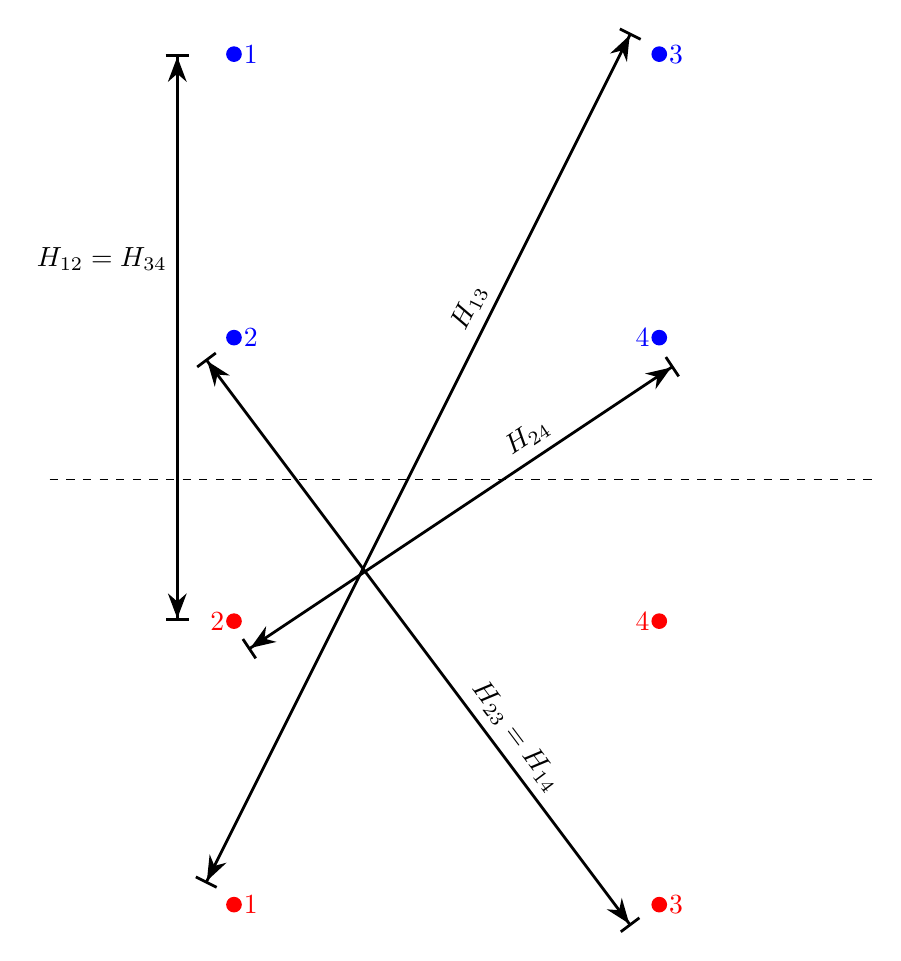
\begin{tikzpicture}[scale=1.8, >=Stealth]
    \coordinate[label={[blue]right:1}] (P1) at (0,3);
    \coordinate[label={[blue]right:2}] (P2) at (0,1);
    \coordinate[label={[blue]right:3}] (P3) at (3,3);
    \coordinate[label={[blue]left:4}] (P4) at (3,1);

    \coordinate[label={[red]right:1}] (I1) at (0,-3);
    \coordinate[label={[red]left:2}] (I2) at (0,-1);
    \coordinate[label={[red]right:3}] (I3) at (3,-3);
    \coordinate[label={[red]left:4}] (I4) at (3,-1);

    \draw[dashed] (-1.3,0) -- (4.5,0);

    \node at (P1) [circle,fill,inner sep=2pt, blue]{};
    \node at (P2) [circle,fill,inner sep=2pt, blue]{};
    \node at (P3) [circle,fill,inner sep=2pt, blue]{};
    \node at (P4) [circle,fill,inner sep=2pt, blue]{};

    \node at (I1) [circle,fill,inner sep=2pt, red]{};
    \node at (I2) [circle,fill,inner sep=2pt, red]{};
    \node at (I3) [circle,fill,inner sep=2pt, red]{};
    \node at (I4) [circle,fill,inner sep=2pt, red]{};

    \draw [{Bar[scale=1.2]Stealth[scale=1.2]}-{Stealth[scale=1.2]Bar[scale=1.2]}, line width=1] ($(I2) + (.1,-.2)$) -- ($(P4) + (.1,-.2)$) node[midway, sloped, above, xshift=12mm] {$H_{24}$};

    \draw [{Bar[scale=1.2]Stealth[scale=1.2]}-{Stealth[scale=1.2]Bar[scale=1.2]}, line width=1] ($(P1) - (.4,0)$) -- ($(I2) - (.4,0)$) node[midway, left, yshift=10mm] {$H_{12} = H_{34}$};

    \draw [{Bar[scale=1.2]Stealth[scale=1.2]}-{Stealth[scale=1.2]Bar[scale=1.2]}, line width=1] ($(I1) + (-.2,.15)$) -- ($(P3) + (-.2,.15)$) node[midway, sloped, above, xshift=20mm] {$H_{13}$};

    \draw [{Bar[scale=1.2]Stealth[scale=1.2]}-{Stealth[scale=1.2]Bar[scale=1.2]}, line width=1] ($(P2) - (.2,.15)$) -- ($(I3) - (.2,.15)$) node[midway, sloped, above, xshift=17mm] {$H_{23} = H_{14}$};

  \end{tikzpicture}
  \caption{Diagrama do sistema, já considerando as simplificações e fora de escala, indicando a distância $H_{ki}$ entre o eletrodo $k$ (em azul) e a imagem do eletrodo $i$ (em vermelho).}
  \label{fig:d3}
\end{figure}


\end{document}
